\documentclass[11pt,a4paper]{article}

\usepackage[left=2cm,text={17cm,24cm},top=3cm]{geometry}
\usepackage[czech]{babel}
\usepackage[utf8]{inputenc}
\usepackage[T1]{fontenc}

\usepackage{url}
\usepackage{tikz}
\usepackage{float}
\usepackage{xcolor}
\usepackage{siunitx}
\usepackage{amsmath}
\usepackage{accents}
\usepackage{comment}
\usepackage{listings}
\usepackage{csquotes}
\usepackage{hyperref}
\usepackage{textcomp}
\usepackage{amsfonts}
\usepackage{breakurl}
\usepackage{etoolbox}
\usepackage{graphicx}
\usepackage{multicol}
\usepackage{multirow}
\usepackage{indentfirst}
\usepackage{supertabular}
\usepackage[titles]{tocloft}
\usepackage{dirtytalk}
\usepackage{pdfpages}
\usepackage[bottom]{footmisc}

\def\UrlBreaks{\do\/\do-} % URL breaking characters

\newcommand{\red}[1]{\textcolor{red}{#1}} % \red{text in red}
\newcommand{\blue}[1]{\textcolor{blue}{#1}} % \blue{text in blue}
\newcommand{\TODO}{\textbf{\textcolor{red}{TODO}}} % red bold TODO
\newcommand{\tilda}{\raisebox{0.5ex}{\texttildelow}} % command \tilda for '~' character

\renewcommand{\cftdot}{}

\setlength\parindent{0pt} % do NOT indent
\graphicspath{{img/}} % path to images

\patchcmd{\thebibliography}{\section*{\refname}}{}{}{}



\makeatletter
\newcommand\xleftrightarrow[2][]{%
  \ext@arrow 9999{\longleftrightarrowfill@}{#1}{#2}}
\newcommand\longleftrightarrowfill@{%
  \arrowfill@\Leftarrow=\Rightarrow}
\makeatother

\begin{document}

\begin{titlepage}

    \begin{center}
        % FIX: lines must end with '%', if not then it will result in an incorrect centering
        \vfill {%
            \Huge{%
                \textsc{%
                    Fakulta informačních technologií\\[3mm]%
                    Vysoké učení technické v~Brně%
                }%
            }%
        }%

        \hfill\\[15mm]

        \begin{figure}[!h]
            \centering
            
\includegraphics[scale=0.3]{vutbr-fit-logo.eps}
        \end{figure}

        \hfill\\[10mm]

        \Huge{
            \textbf{
                TIN
            }
        }

        \hfill\\[-10mm]

        \huge{
            \textbf{
                Teoretická informatika
            }
        }

        \hfill\\[10mm]

        \LARGE{
            \textbf{
                3. domácí úloha
            }
        }
        \vfill

    \end{center}

        \Large{
            Attila Lakatos (xlakat01)\hfill \today
        }

\end{titlepage}

\setlength{\parskip}{0pt}
    \hypersetup{hidelinks}\tableofcontents
\setlength{\parskip}{0pt}

\newpage

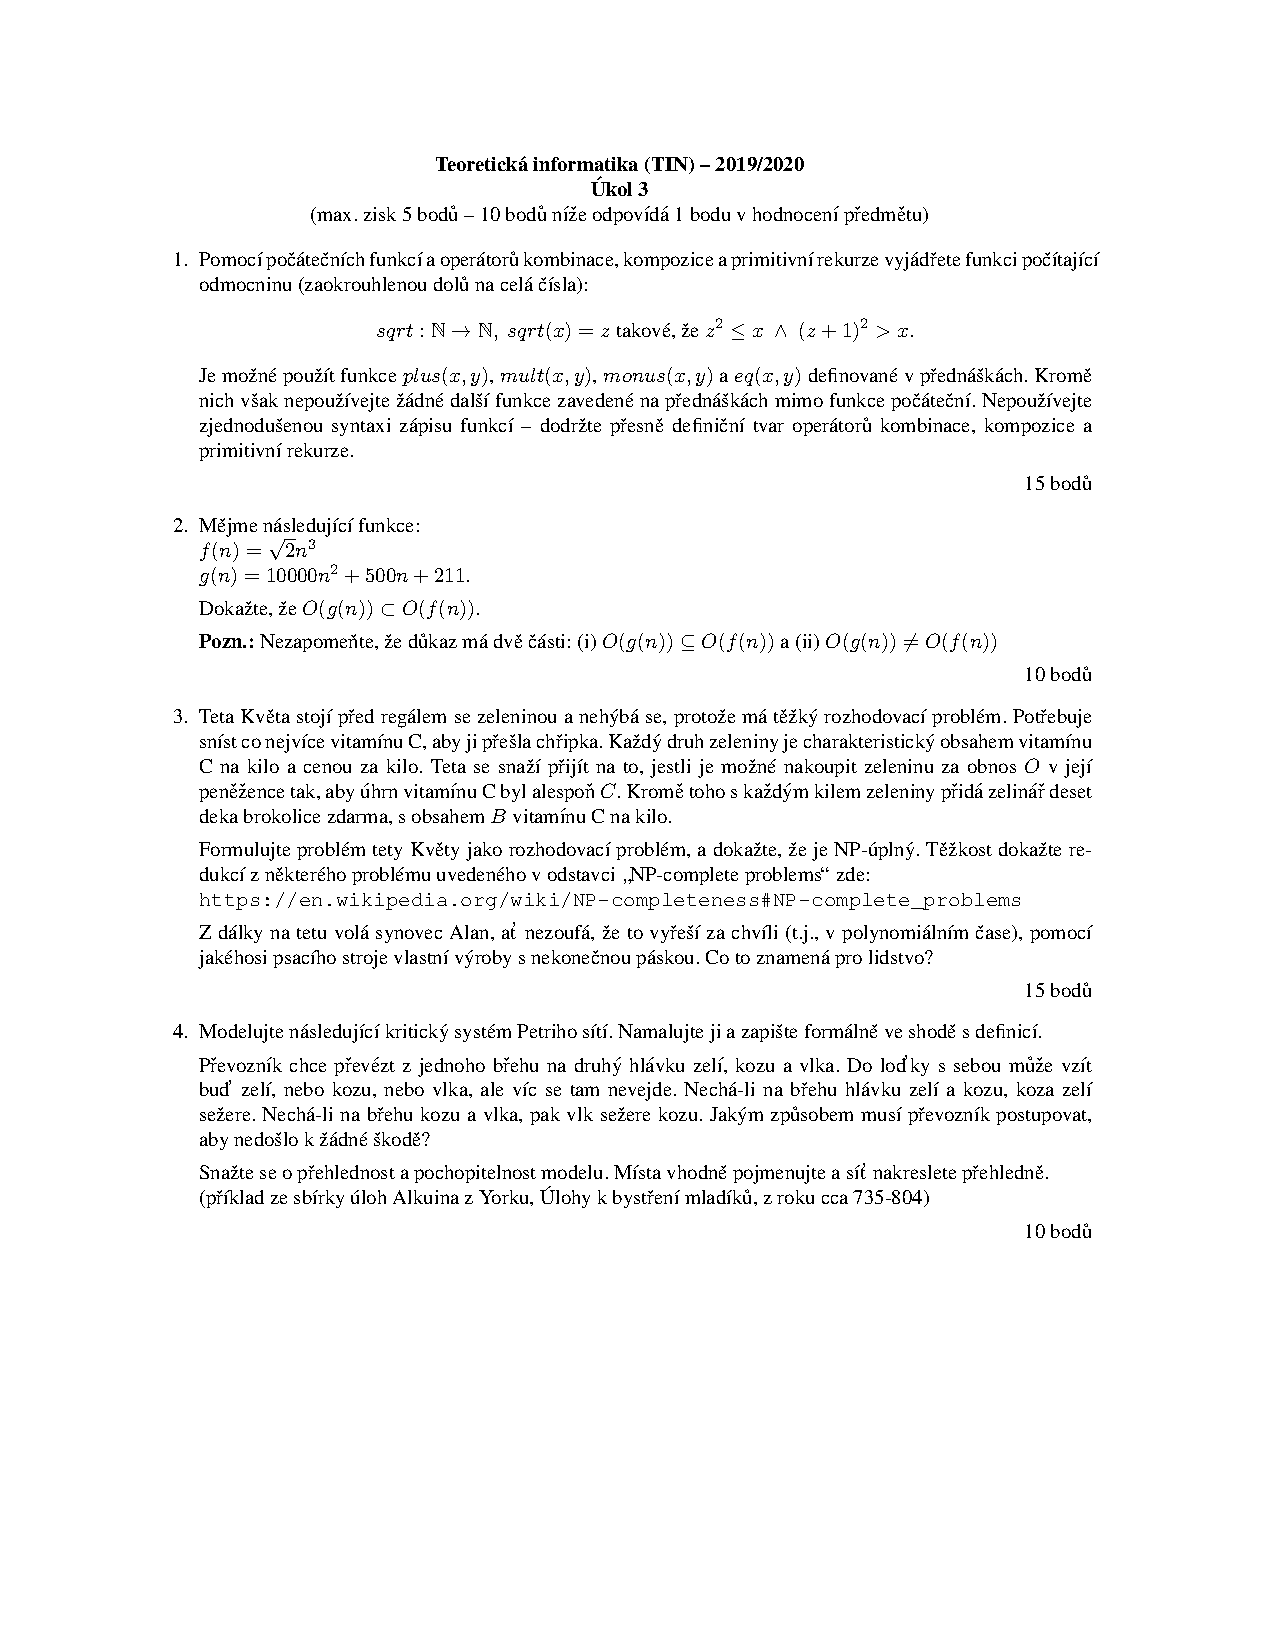
\includepdf[pagecommand={},width=1.5\textwidth]{zadanie3.pdf}

% Task 1
\section{1.úloha}
\newpage

% Task 2
\section{2.úloha}
Zostrojme si graf funkcie pre $ f(n) = \sqrt{2} n^3$ a pre $ g(n) = 10000n^2 + 500n + 211 $. \\

\begin{figure}[H]
    \centering
	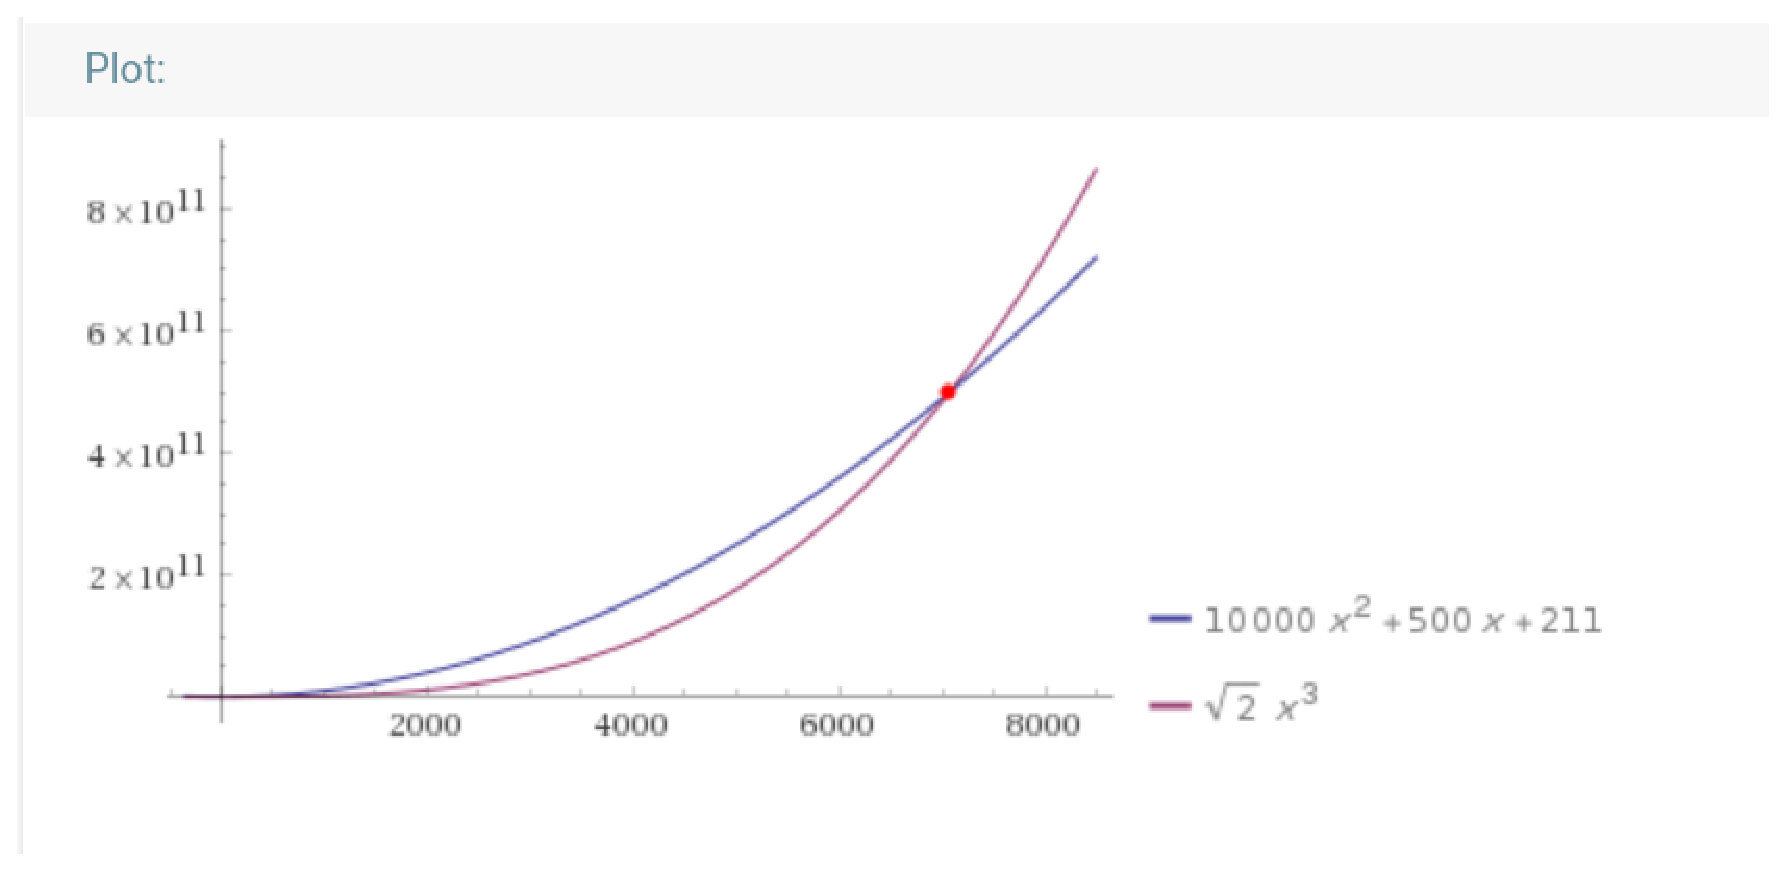
\includegraphics[width=\textwidth]{2plot.eps}
    \caption{f(x) a g(x)}
    \label{2plot}
\end{figure}


Diskriminant $D$ kubickej rovnice $ \sqrt{2}n^3 -10000n^2 -500n -211 = 0$ vypočítame podľa vzťahu: 
\begin{align*}
    D & = 18abcd -4b^3d + b^2c^2 - 4ac^3 - 27a^2d^2 \\
    D & = 18*\sqrt{2}*(-10000)*(-500)*(-211) & \\
      & -4*(-10000)^3*(-211) & \\
      & +(-10000)^2*(-500)^2 & \\ 
      & -4*\sqrt{2}*(-500)^3 & \\
      & -27*\sqrt{2}^2*(-211)^2 \\
    D &= -8.1902*10^{14}
\end{align*}

$D < 0$, rovnica má jeden reálny koreň.

Na obrázku \ref{2plot} vidíme priesečník grafov dvoch funkcí. Riešením rovnice $ f(x) = g(x) $ získame x-ové súradnice priesečníkov grafov,\footnote{Nástroj na výpocět kubickej rovnice: https://www.wolframalpha.com/widgets/view.jsp?id=3f4366aeb9c157cf9a30c90693eafc55} ich dosadením do predpisu funkcie získame y-ové súradnice.

\label{2equation}
\begin{align*}
    f(n) & = g(n) \\
   \sqrt{2} n^3 - 10000n^2 -500n -211 & = 0 \\
    n & = 7071.1
\end{align*}

\newpage
\paragraph{Dôkaz:}\mbox{{}}\\
\begin{enumerate}
    \item Z výsledkov rovnice a z grafu funkcí(Obr. \ref{2plot}) vyplíva, že od $n = 7072$ je $ f(n) > g(n)$. Obidve funkcie majú rovnaký definičný obor, teda môžeme povedať, že $ O(g(n)) \subseteq O(f(n)) $.

    \item Vieme, že výsledkom rovnice je len jeden jediný realný koreň(D < 0), a je naprosto zrejmé, že od $ n = 7072 $ sa tieto dve funkcie nikde inde nerovnajú, tak potom $ O(g(n)) \neq O(f(n)) $.
\end{enumerate}

\paragraph{Teda:}\mbox{{}}\\
$ O(g(n)) \subseteq O(f(n)) \land O(g(n)) \neq O(f(n)) \Rightarrow O(g(n)) \subset O(f(n)) $.


\newpage
% Task 3
\section{3.úloha}
Pre dôkaz ťažkosti problem tety kvety použijeme polynomiálnu redukciu z problému "Subset sum problem", ktorý je mimochodom NP úplny problem.

\textbf{Tento problem si vyjádrime zápisom: } \\

$\sum\limits_{i=1}^{n} (c_i + B) * x_i \geq C \land \sum\limits_{i=1}^{n} o_i * x_i \leq 0 $ pre $  x_i \in \{0, 1\} $, kde \\

$ x_i $ je informácia, či sa (ne)bude táto položka nachádzať v nákupnom košíku, \\

$ o_i $ je cena 1 kg danej zeleniny, \\

$ n $ je veľkosť množiny (do toho sa započíta celková hmotnosť zeleniny v obchode okrem brokolice) \\

$ C $ vyjadruje minimalné požadované množstvo vitaminov C \\

$ B $ množstvo vitaminu C v 0,1kg brokolice \\

$c_i$ je množstvo vitaminu C v 1 kg danej zeleniny \\

$ i $ je pomocná premenná \\

\textit{Problem subset sum obecne:} Je daná množina prirodzených čísel $ M = \{n1, n2, ..., n_r\} $ a číslo $k$. Rozhodovací problém sa spýta, či je možné vybrať z M podmnožinu N tak, že súčet čísel N je rovno k. \footnote{Subset sum problem: https://www.algoritmy.net/article/7682/Subset-sum-\%E2\%86\%92-Deleni-koristi}

\textbf{Problem formulujeme nasledujúcim zápisom:} \\

$ \sum\limits_{i=1}^{n} v_i * y_i = k $ pre $ y_i \in \{0, 1\}$

Nasleduje redukcia Subset sum problemu na Problem tety kvety. V prvodem rade vytvoríme instanciu problému tety kvety nasledujúcim spôsobom:

\begin{align*}
    (c_i + B) = o_i = v_i \\
    C = O = k
\end{align*}

Túto redukciu bude vykonať úplny DTS, jeho zložitosť bude iste spadať do triedy $O(n^l)$.
Odpoveď Áno/Nie na vytvorený problem tety kvety potom súvisí s odpoveďou na pôvodný problem: \\

    \begin{align*}
        \left.
        \begin{array}{r@{}l}
            \sum\limits_{i=1}^{n} (c_i + B) x_i \geq C & \iff \sum\limits_{i=1}^{n} v_i * x_i \geq k \\
            \sum\limits_{i=1}^{n} o_i * x_i \leq 0 & \iff \sum\limits_{i=1}^{n} v_i * x_i \leq k
        \end{array}
        \right\rbrace
        \begin{array}{r@{}l}
            \iff \sum\limits_{i=1}^{n} v_i * x_i = k \hspace{0,3cm}pre \hspace{0,2cm} x_i =\in \{0, 1\} 
        \end{array}
    \end{align*}

To znamená, že keď najdeme vektor x takový, ktorý vyhovuje problému tety kvety, potom ten istý vektor x je aj riešením \textbf{subset problemu} a zároveň odpoveď zo \textbf{subset problemu} je Áno. Inak (ak sme takýto vektor nenašli) - neexistuje podmnožina pre danú množinu, kde súčet by bol rovno číslu $k$, dostaneme odpoveď Nie. \\

Správnosť odpovedí ukážeme ukážeme v polynomiálnom čase - sčítame obsah vitaminu C, ceny a hodnoty, ktoré potom budeme porovnávať so stanovenými hranicami.


\paragraph{Pre ľudstvo znamená:}\mbox{{}}\\
\begin{enumerate}
    \item Stroj v batohu je deterministický - Stroj v batohu dokáže vyriešiť v polynomiálnom čase problem s exponenciálnou zložitosťou: $ P = NP $. Toto zistenie by viedlo k najdení rychlejších algoritmov na vyriešenie NP úplnych úloh. \\
    \item Stroj v batohu je NEdeterministický - Alan použil tzv. Turingov stroj. Definícou tohto teoretického stroja ukázal univerzialny prostriedok na vyjádrenie rôznych algoritmov. Pomocou tohoto  nedeterministického stroje je možné vyriešiť aj problém s exponenciálnou zložitosťou v polynomialnom čase. Ak existuje správne riešenie , tak sa nachádza medzi všetkými nedeterministickými možnými riešeniami, ktoré uhádne a potom stačí overiť jeho správnosť.
\end{enumerate}


\newpage
% Task 4
\section{4.úloha}

Jednoduchá reprezentácia komplexného systému si vyžaduje rozdelenie zadania úlohy na mänšie části. Z tohto dôvodu som sa rozhodol rozdeliť riešenie danej úlohy na 4 části, ktoré sú nasledujúce:
\begin{enumerate}
    \item Prechod z ľavej strany na pravú (Obrázok \ref{fig:pn1})
    \item Prechod z pravej strany na ľavú (Obrázok \ref{fig:pn2})
    \item Vlk zožerie kozu/koza zožerie zelí na ľavej strane, keď prievozník je na pravej strane (Obrázok \ref{fig:pn3})
    \item Vlk zožerie kozu/koza zožerie zelí na pravej strane, keď prievozník je na ľavej strane (Obrázok \ref{fig:pn4})
\end{enumerate}

Výsledná Petriho sieť vyzerá následovne\cite{AA}: \\
\begin{align*}
    N = (P, T, F, W, K, M_0)
\end{align*}

Množina miest \textbf{P}:
\begin{itemize}
    \item \textbf{vlk1} - vlk sa nachádza na ľavej strane, \textbf{vlk2} - vlk sa nachádza na pravej strane
    \item \textbf{koza1} - koza sa nachádza na ľavej strane, \textbf{koza2} - koza sa nachádza na pravej strane
    \item \textbf{zelí1} - zelí je na ľavej strane, \textbf{zelí2} - zelí je na pravej strane
    \item \textbf{prievozník1} - prievozník je na lavej strane, \textbf{prievozník2} - prievozník je na pravej strane
\end{itemize}

Množina priechodov \textbf{T}:
\begin{itemize}
    \item \textbf{vlk\_na\_lodi1} - vlk prejde z ľavej strany na pravú, \textbf{vlk\_na\_lodi2} - vlk prejde z pravej strany na ľavú
    \item \textbf{koza\_na\_lodi1} - koza prejde z ľavej strany na pravú, \textbf{koza\_na\_lodi2} - koza prejde z pravej strany na ľavú
    \item \textbf{zelí\_na\_lodi1} - zelí prejde z ľavej strany na pravú, \textbf{zelí\_na\_lodi2} - zelí prejde z pravej strany na ľavú
    \item \textbf{prievozník\_na\_lodi1} - prievozník prejde z ľavej strany na pravú, \textbf{prievozník\_na\_lodi2} - prievozník prejde z pravej strany na ľavú
    \item \textbf{vlk+koza 1} - vlk zožerie kozu na lavej strane, \textbf{vlk+koza 2} - vlk zořerie kozu na pravej strane
    \item \textbf{koza+zelí 1} - koza zožerie zelí na lavej strane, \textbf{koza+zelí 2} - koza zořerie zelí na pravej strane
\end{itemize}

\newcommand{\Cross}{\mathbin{\tikz [x=1.4ex,y=1.4ex,line width=.2ex] \draw (0,0) -- (1,1) (0,1) -- (1,0);}}

Toková relácia  \textbf{F} $ \subseteq (P \Cross T) \cup (T \Cross P) $:
\begin{itemize}
    \item (vlk1, vlk\_na\_lodi1), (vlk\_na\_lodi1, vlk2), (koza1, koza\_na\_lodi1), (koza\_na\_lodi1, koza2), (zelí1, zelí\_na\_lodi1), (zelí\_na\_lodi1, zelí2), (prievozník1, prievozník\_na\_lodi1), (prievozník\_na\_lodi1, prievozník2)
    \item (vlk2, vlk\_na\_lodi2), (vlk\_na\_lodi2, vlk1), (koza2, koza\_na\_lodi2), (koza\_na\_lodi2, koza1), (zelí2, zelí\_na\_lodi2), (zelí\_na\_lodi2, zelí1), (prievozník2, prievozník\_na\_lodi2), (prievozník\_na\_lodi2, prievozník1)
    \item (vlk1, vlk+koza 1), (vlk+koza 1, vlk1), (koza1, vlk+koza 1), (koza1, koza+zeli 1), (koza + zeli 1, koza1), (zeli1, koza+zeli 1), (vlk+koza 1, prievoznik2), (prievoznik2, vlk+koza 1), (koza+zeli 1, prievoznik2), (prievoznik2, koza+zeli 1)
    \item (prievoznik1, vlk+koza 2), (vlk+koza 2, prievoznik1), (prievoznik1, koza+zeli 2), (koza+zeli 2, prievoznik1), (vlk+koza 2, vlk2), (vlk2, vlk+koza 2), (koza2, vlk+koza 2), (koza+zeli 2, koza), (koza2, koza+zeli 2), (zeli2, koza+zeli 2)
\end{itemize}

\textbf{W} : $ F \rightarrow \mathbb N  \backslash \{0\}$ je ohodnocení hran grafu určujúci kladnú váhu každej hrany siete
\begin{itemize}
    \item Každá hrana má ohodnocenie \textbf{1}.
\end{itemize}

\textbf{K} : $ P \rightarrow \mathbb N \cup \{w\} $ je zobrazenie určujúci kapacaitu každého miesta
\begin{itemize}
    \item Kapacita každého miesta je \textbf{1} (maximálne 1 vlk, 1 koza, 1 zelí, 1 prievozník)
\end{itemize}

$\mathbf{M_0} : P \rightarrow \mathbb N \cup \{w\} $ je počiatočné značenie miest Petriho siete takové, že $ \forall p \in P: M_0(p) \leq K(p) $
 
\begin{enumerate}
    \item Počiatočná konfigurácia jednotlivých značiek závisí na zadáni úlohy(z čoho mimochodem nie je jasné, že na ktorej strane sa nachádzajú jednotlivé entity na začiatku). Defaultná konfigurácia je taková, že každá entita z množiny entit {vlk, koza, zelí, prievozník} je na ľavej strane.
\end{enumerate}

\begin{figure}[H]
    \centering
	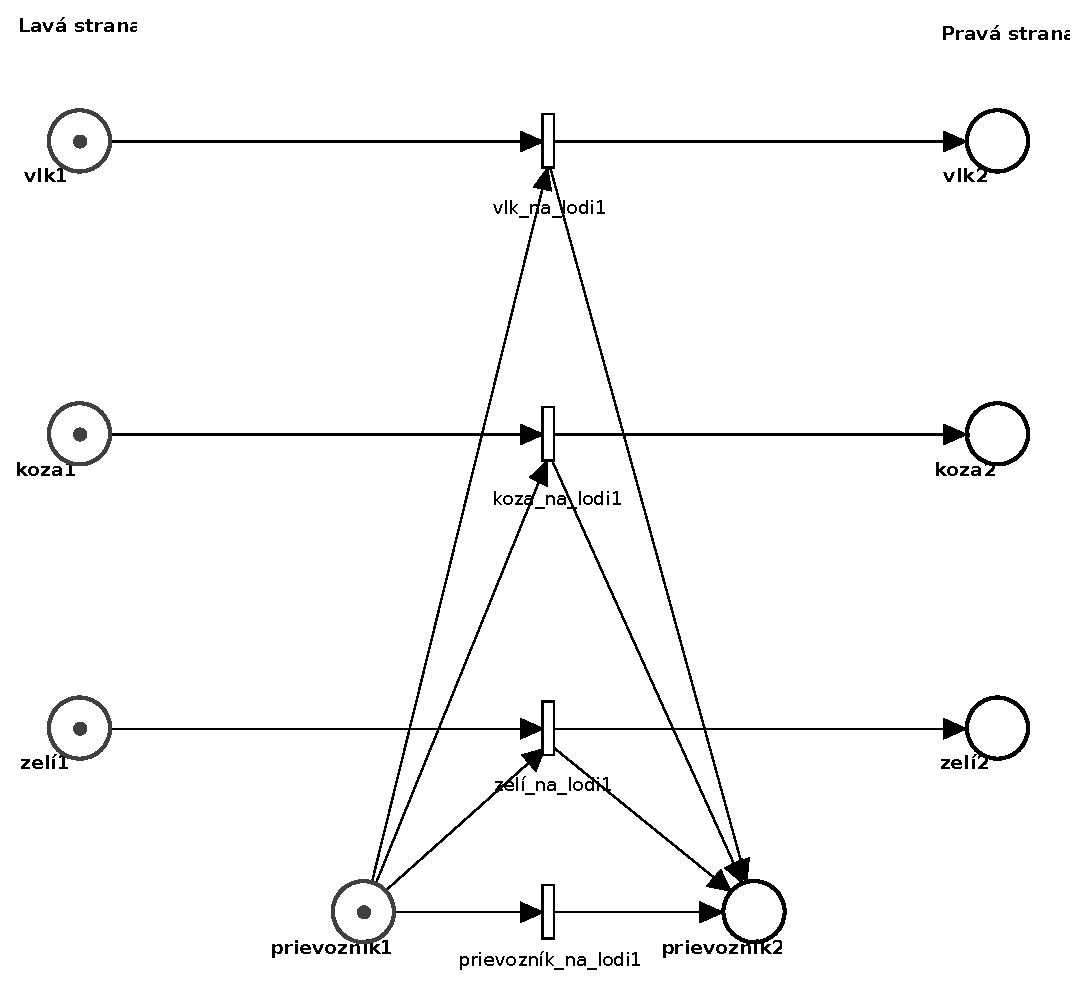
\includegraphics[width=0.6\textwidth]{pn1NEW.eps}
    \caption{Ľavá strana $\protect\Rightarrow$ Pravá strana}
    \label{fig:pn1}
\end{figure}

\begin{figure}[H]
    \centering
	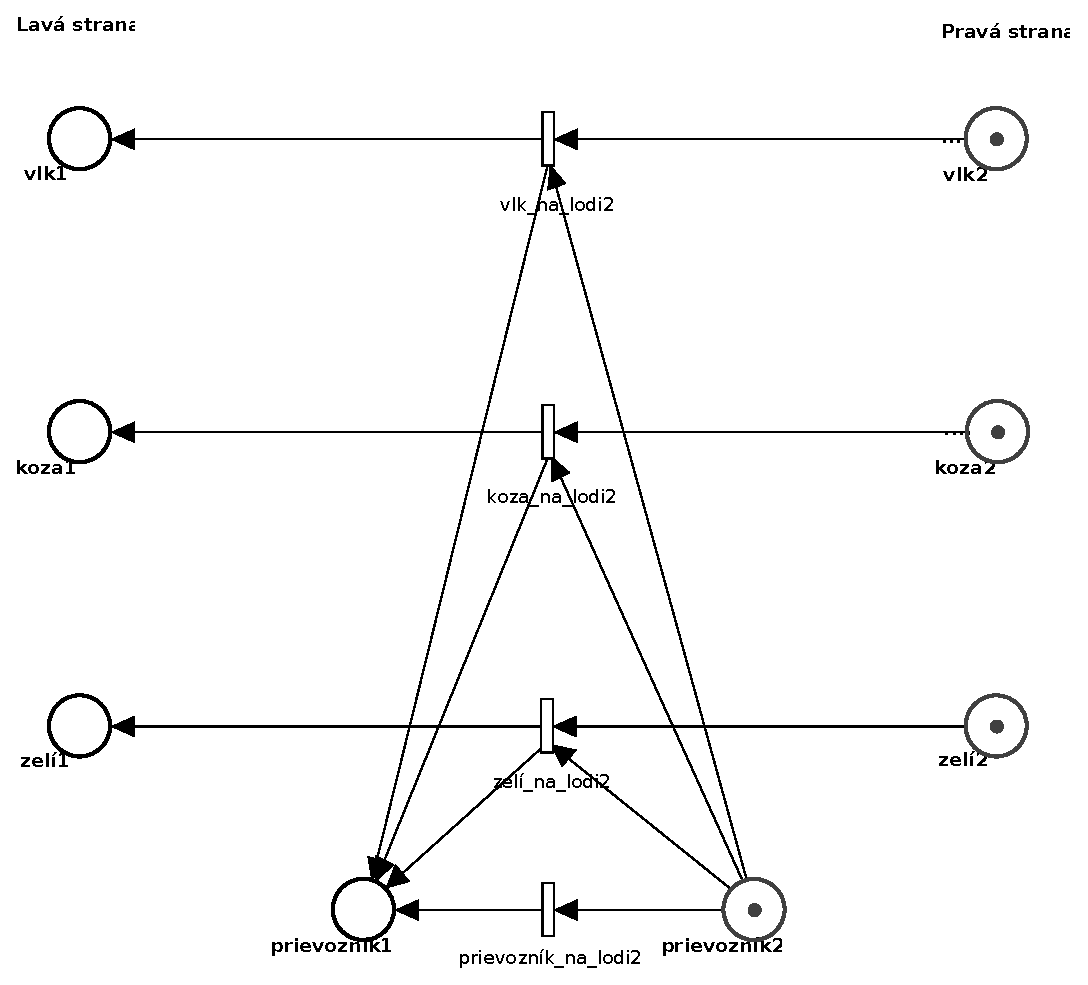
\includegraphics[width=0.6\textwidth]{pn2NEW.eps}
    \caption{Pravá strana $\protect\Rightarrow$ Ľavá strana}
    \label{fig:pn2}
\end{figure}

\begin{figure}[H]
    \centering
	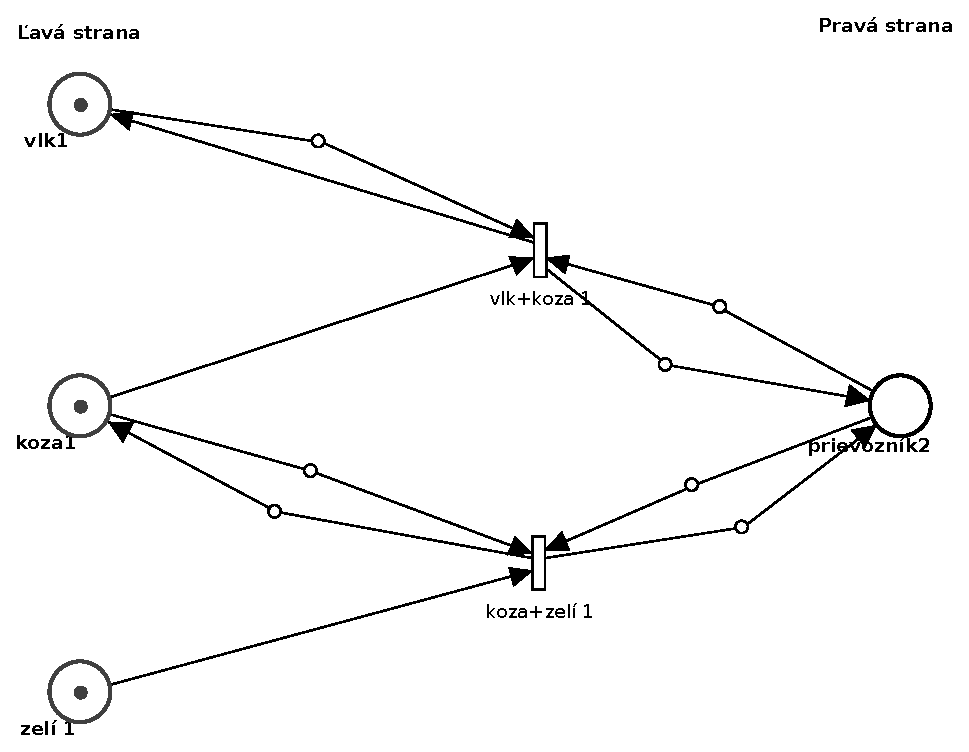
\includegraphics[width=0.6\textwidth]{pn3NEW.eps}
    \caption{Koza zožerie zelí alebo vlk zožerie kozu na ľavej strane, keď prievozník je na pravej strane}
    \label{fig:pn3}
\end{figure}

\begin{figure}[H]
    \centering
	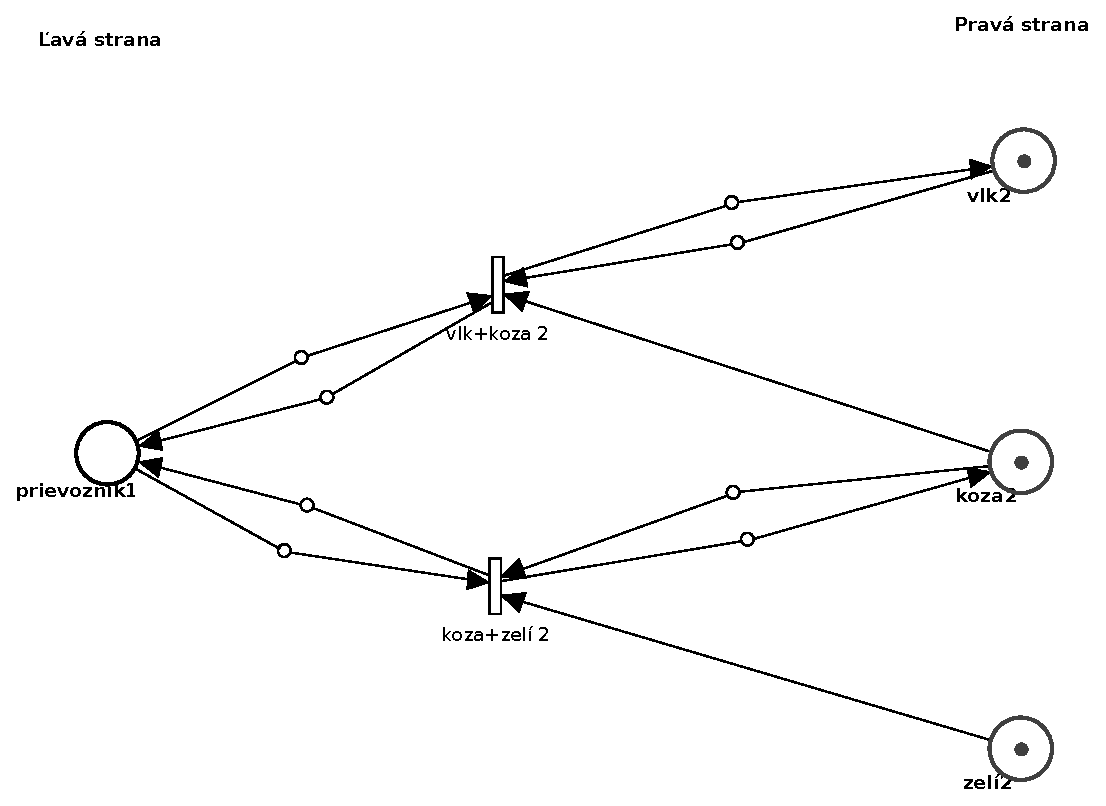
\includegraphics[width=0.6\textwidth]{pn4NEW.eps}
    \caption{Koza zožerie zelí alebo vlk zožerie kozu na pravej strane, keď prievozník je na ľavej strane}
    \label{fig:pn4}
\end{figure}

\newpage

\section{Literatura}
\bibliographystyle{czechiso}
\begin{flushleft}
    \bibliography{quotation}
    \end{flushleft}

\end{document}
